\documentclass{beamer}
\usepackage{config}

%Information to be included in the title page:
\title[CLI]{Les terminaux de commande ou CLI}
\author{Florian Legendre}
\institute{Université de Poitiers}
\date{Année 2020 - 2021}
\logo{
\includegraphics[scale=0.1]{UP.png}}


%%% ============================================================= %%%
%%% ====================== Début des diapos ===================== %%%
%%% ============================================================= %%%

\begin{document}

\frame{\titlepage}

\begin{frame}
\frametitle{Table of Contents}
\tableofcontents[hideallsubsections]
\end{frame}


%% --------------------- %%
%%        SECTION        %%
%% --------------------- %%
\AtBeginSection[]
{
  \begin{frame}
    \frametitle{Table of Contents}
    \tableofcontents[sectionstyle=show/hide,subsectionstyle=show/show/hide]
  \end{frame}
}
\section{Présentation des CLI}

% Subsection:
\subsection{Qu'est qu'une CLI?}

\begin{frame}[fragile]
\frametitle{Notion d'invite de commande}
Au commencement de l'ordinateur était la CLI (Command Line Interface) aussi connue sous le nom de terminal de commande. Quand on ouvre un terminal de commande on se retrouve face à une invite de commande:

\begin{mdframed}[style=Bash]
\begin{lstlisting}[style=Bash, caption={Une "invite" de commande}]
crex@crex:~$ 
\end{lstlisting}
\end{mdframed}

Une invite de commande vous "invite" à commander votre ordinateur. Vous pouvez le voir comme un serveur de restaurant à qui vous passeriez une commande: "fais ceci pour moi... Et ça...", etc.

\end{frame}

% Subsection:
\subsection{Quel lien avec les UI?}

\begin{frame}[fragile]
\frametitle{Lien commandes/GUI}
Les GUI (Graphical User Interface) sont des traductions graphiques de commandes.\\

Les GUI remplacent le "garçon du café" par un tableau de bord d'avion: boutons, manettes (sliders), etc.\\
\bigskip

\begin{tabular}{  m{9em} m{5em} m{10em}  }
    
    \begin{center}
        
\includegraphics[scale=0.2]{images/Jenkins_logo.png}
    \end{center}
    & 
    \textbf{FIGHT!}
    &
    
    \begin{center}
        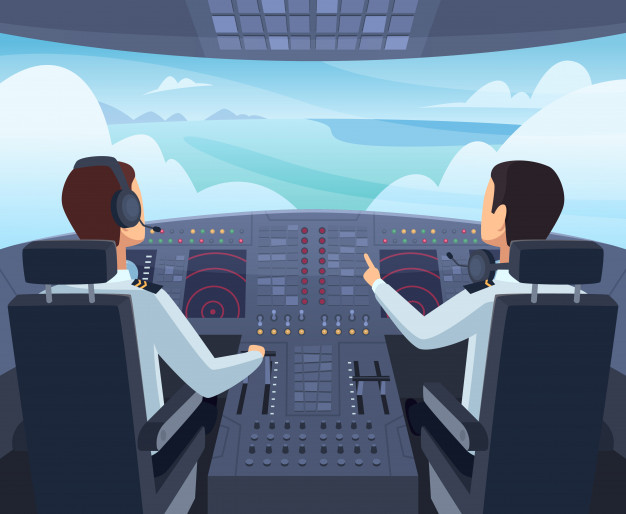
\includegraphics[scale=0.2]{images/cockpit.jpg}
    \end{center} \\
    
\end{tabular}

\end{frame}


% Subsection:
\subsection{Comparaison CLI/GUI}

\begin{frame}[fragile]
\frametitle{Qui gagne?}

Comme souvent en informatique (voire en ingénieurie ou encore... La vie?) on échange généralement des avantages contre des inconvénients.
\bigskip

\tiny
\begin{tabular}{ | m{20em} | m{20em} | }
    \hline
    \textbf{Les CLI} & \textbf{Les GUI}\\
    \hline
    
    \begin{itemize}
        \item[+] Des fonctionnalités plus puissantes que les GUI
        \item[+] Des bugs en moins
        \item[+] Rapide à lancer et utiliser
        \item[+] En cas d'erreur les messages sont généralement clairs et explicites
        \item[-] Il faut connaître des mots-clefs/des syntaxes...
        \item[-] Il faut lire un manuel si on ne connaît pas le mot-clef/la syntaxe pour obtenir ce qu'on veut
        \item[-] Pour des besoins très complexes (matLab) la quantité de mots-clefs/syntaxes peut devenir énorme
    \end{itemize}
    & 
    \begin{itemize}
        \item[+] Sont devenues très intuitives avec le temps
        \item[+] Permettent de répondre à 95\% des services qu'on souhaite obtenir très simplement et sans mots-clés/syntaxes
        \item[+] Rendent accessibles des applications complexes
        \item[-] Peuvent contenir des bugs liées à l'interface
        \item[-] En cas d'erreur les messages sont généralement peu clairs si tant est qu'on y a même accès
        \item[-] Peuvent être lentes à lancer
        \item[-] Gourmandes en ressources ordinateur
    \end{itemize} \\
    
    \hline
\end{tabular}
\normalsize

\end{frame}



%% --------------------- %%
%%        SECTION        %%
%% --------------------- %%
\AtBeginSection[]
{
  \begin{frame}
    \frametitle{Table of Contents}
    \tableofcontents[sectionstyle=show/hide,subsectionstyle=show/show/hide]
  \end{frame}
}
\section{Quelques commandes de Bash}

% Subsection:
\subsection{Naviguer dans le terminal}

\begin{frame}[fragile]{Naviguer dans une arborescence de fichiers}
Un terminal de commande nous place à un endroit de notre arborescence des fichiers qu'il appelle \$HOME ou encore '$\sim$'. Depuis cet endroit il est possible de se déplacer dans l'arborescence de fichiers en utilisant deux commandes, 'ls' et 'cd':\\

\begin{itemize}
    \item ls => \textbf{L}i\textbf{S}te les dossiers et fichiers à l'endroit où vous vous trouvez dans l'arborescence
    \item cd <nom\_du\_dossier> => \textbf{C}hanger de \textbf{D}ossier vers le dossier indiqué
    \item cd .. => remonter d'un dossier dans l'arborescence
    \item cd ../../ => remonter de deux dossiers
    \item cd - => revenir au dossier précédent
    \item cd /c => Aller dans le dossier C:\textbackslash
\end{itemize}
\end{frame}

\begin{frame}{Copier-coller et chemins Windows}
Les traditionnels raccourcis "Ctrl+C, Ctrl+V" ne marchent pas dans un terminal Bash (ils ont une autre signification pour Bash). Le raccourci dépend de votre système (Ctrl+Insert et Shift+Insert pour certaines personnes.) Ce qui marchera toujours c'est un clic droit + copier ou coller.\\
\bigskip

\textbf{IMPORTANT:} Entourez tous vos chemins Windows de guillemets dans Bash! Exemple: \textit{ls "C:\textbackslash mon\textbackslash super\textbackslash chemin"}
\end{frame}

% Subsection:
\subsection{Ressources pour aller plus loin}

\begin{frame}[fragile]
\frametitle{Ressources pour aller plus loin}
Les commandes présentées ci-dessus nous suffiront largement pour notre présentation de git. Bien évidemment il ne s'agit que d'un très très mince échantillon des commandes disponibles sur Bash (ou git Bash). Pour en découvrir davantage je vous recommande l'excellent jeu:
\bigskip

\begin{center}
    \url{https://overthewire.org/wargames/bandit/}
\end{center}
\bigskip

Arrivez au niveau 10 et vous serez déjà bilingue Français/Bash!

\end{frame}


\end{document}